\section{Graphics}

Visualizing the game consists of managing several graphical areas, including XML layout, drawing the maps, towers, mobs, projectiles, animations, tooltips and the towers being dragged across the screen while placing them.

\subsection{XML layout}

Since the class MenuGame is where the progression map is drawn, it does not have a predefined layout. Instead of getting the layout from an XML file, View objects are created and attached to MenuGame during runtime. This activity uses canvas, which will be further explained in the Draw section, to show images on the screen. 

The main menu of the game and all the buttons have been positioned using the XML editor but the customization of the buttons has been drawn using Adobe Photoshop. As shown in figure ~\ref{fig:xmlLayout}, the main menu contains a Relative Layout which contains a Table Layout with five buttons: StartGame, Help, Options, Credits and Exit. 

%------------------------------
%- Image XML Layout
%------------------------------
\begin{figure}[h]
\begin{center}
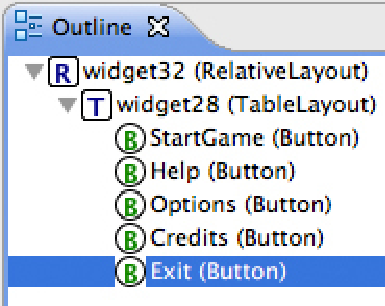
\includegraphics[scale=0.7]{pics/chapters/chapter4/xmllayout}
\end{center}
\caption{Outline view of the layout editor in eclipse}
\label{fig:xmlLayout}
\end{figure}
%------------------------------

Different properties can be set for the elements of the layout. As an example, the Relative Layout has a background image set in the property window. Table Layout has different alignment settings and the buttons have a Background property which contains a reference to a new XML file. This allows different states on the buttons, and the states indicates if the user is hovering over, presses and releases the button. 

%---------------------------------------------
%- Image property window layout editor eclipse
%---------------------------------------------
\begin{figure}[h]
\begin{center}
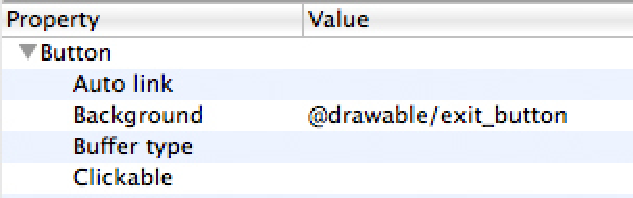
\includegraphics[scale=1]{pics/chapters/chapter4/exitbuttonref}
\end{center}
\caption{Property window of the layout editor in Eclipse.}
\label{fig:propWindowLayoutEditorEclipse}
\end{figure}
%---------------------------------------------

The XML-file (exit\_button.xml), which is referenced from the Exit button's Background property in the main menu, contains the code shown in figure ~\ref{fig:codeExXMLExitButton}.
\clearpage
%------------------------
%- Code snippet exit button XML
%------------------------
\begin{figure}[htb]

\begin{small}
\verbatiminput{code/xmlExitButton.java}
\end{small}

\caption{Caption for exit button}
\label{fig:codeExXMLExitButton}
\end{figure}
%------------------------

Depending on the state of the button, different images are shown.

%-----------------------
%- Image of exit button
%-----------------------
\begin{figure}[h]

\begin{center}

\includegraphics[scale=1]{pics/chapters/chapter4/exitbutton}
\end{center}

\caption{The exit button. To the left, not pressed. To the right, pressed.}
\label{fig:exitButtonPressed}
\end{figure}
%-----------------------

\subsection{Draw}

The graphics are handled by the GameView class, which corresponds to both view and controller in the model-view-controller pattern. GameView extends SurfaceView and implements SurfaceHolder.callback() which is called from the main game thread (GameThread). This is done to provide synchronization with the drawing and all values in the game that is being updated. 

In the GameView class there is also a method called fillBitmapCache(), which is invoked when the class is created. This method stores all the images that is being used in a cache, to prevent performance issues occurring due to excessive access to the resources of the application. The cache is implemented with a HashMap using the generated resource identifiers as keys. This ensures images are only loaded once.
\clearpage
%---------------------
%- Image show money
%---------------------
\begin{figure}[here]
\begin{center}
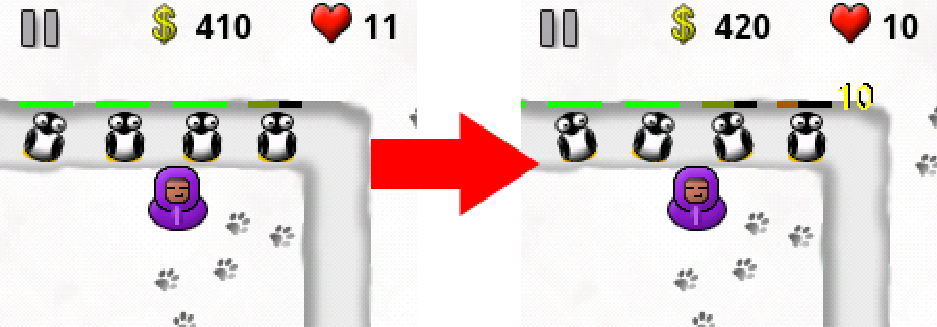
\includegraphics[scale=1]{pics/chapters/chapter4/showmoney}
\end{center}
\caption{Screenshot of a mob dying.}
\label{fig:dyingMob}
\end{figure}
%---------------------

When a mob dies, it is removed from the list of living mobs in the class GameModel and is added to the list of dead mobs called mShowRewardForMob. All of this happens in updateModel() which updates GameModel. The methods updateModel() and onDraw() are frequently called from the game thread. This keeps all values and the canvas up to date which brings the game to life.

The method drawRewardAfterDeadMob loops through all the dead mobs and draws the text with the amount of money you get for killing that mob. The method uses the y-coordinate from the dead mob's last position to know where to draw the text. The text moves upwards by increasing the y-coordinate 12 frames before the dead mob is removed from the list and the method completes. As shown in figure ~\ref{fig:codeExDrawMoney} .

%--------------------------
%- Code snippet draw money
%--------------------------
\begin{figure}[htb]

\begin{small}
\verbatiminput{code/drawMoney.java}
\end{small}

\caption{Example of how to draw graphic to the screen}
\label{fig:codeExDrawMoney}
\end{figure}
%--------------------------

\subsection{Animation}

Animating in Canvas is done by switching bitmaps with regular intervals. One of the animations is the water splash animation at the end of the map. When a mob reaches the final checkpoint it looks like the water splashes up in the air and falls back down again in a smooth manner. This is achieved by showing four images in a sequence. 

%---------
%- Image mob water splash
%----------
\begin{figure}[here]
\begin{center}
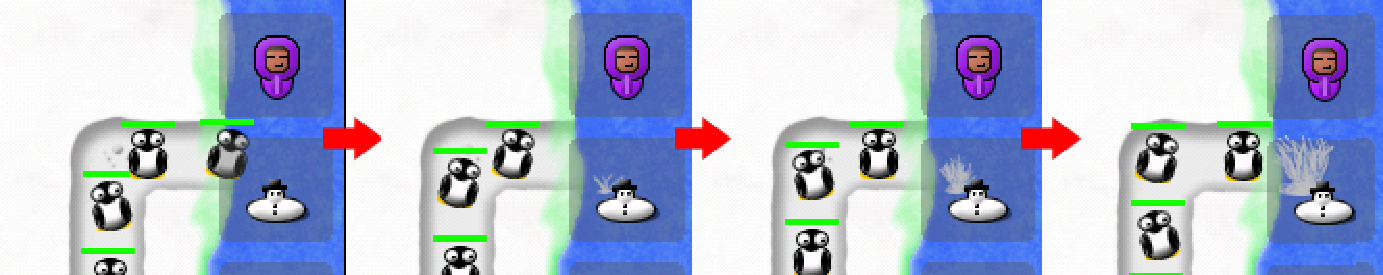
\includegraphics[scale=0.6]{pics/chapters/chapter4/splash2}
\end{center}
\caption{Screenshot of water splash animation}
\label{fig:waterSplashAnimation}
\end{figure}
%----------

The code in figure ~\ref{fig:codeExDrawWaterSplash} shows how animation is solved in practice. A variable keeps track of how many times the animation has been showed, and is used to determine what image will be drawn to the screen. Drawing different images in different intervals of this variable creates the effect of an animation. The water splash animation runs over 25 frames, showing the four different splash images in a sequence. 

%---------
%- Code snippet draw water splash
%---------
\begin{figure}[htb]

\begin{small}
\verbatiminput{code/drawWaterSplash.java}
\end{small}

\caption{Caption for draw water splash..}
\label{fig:codeExDrawWaterSplash}
\end{figure}
%---------

\subsection{Menus}

Apart from the main menu that is defined in an XML-file, in-game menus are also implemented and updated in the method onDraw(). There are three different types of in-game menus: The pause-, defeat- and victory-menu. When the pause button on the top left corner on the screen is pressed, the game is paused and the pause menu appears. The game can also be paused when the back button on the device is pressed.

%---------------------------
%- Image In-game pause menu
%---------------------------
\begin{figure}[h]
\begin{center}
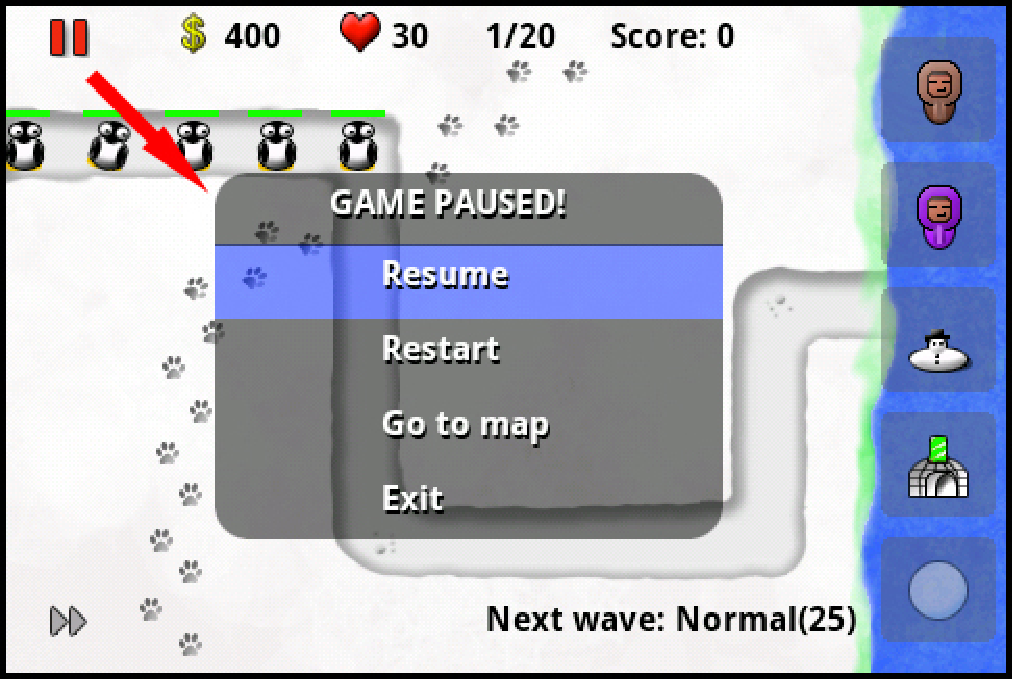
\includegraphics[scale=0.6]{pics/chapters/chapter4/in-gamePauseMenu}
\end{center}
\caption{Screenshot of in-game pause menu.}
\label{fig:ingamePauseMenu}
\end{figure}
%---------------------------

The menu shown in figure ~\ref{fig:ingamePauseMenu} contains five transparent images with some text on top of them. The images behind "Resume", "Restart", "Go to map" and "Exit" also exist with a blue background. These blue images are used when the user keeps his finger over the button, highlighting it. The user can also drag or swipe his finger over the buttons. The buttons are highlightened depending on the current position of the user input.  It is only when the finger is released from the screen that a button is logically pressed. Handling user input this way prevents faulty user input, increasing the usability of the game.

\subsection{Tower placement}

Placing towers is done by touching one of the corresponding buttons on the right side of the screen, and then dragging the tower to the game field. When the player releases his finger, the tower is built and money is withdrawn. Every tower is taking up 32x32 pixels of the screen but the player cannot put towers wherever he wants. The game field is divided into a grid of squares 16x16 pixels. There is no grid painted on the screen. Instead of showing the grid visually, the towers will snap into the positions on the game field where they can be placed. It is not possible to build towers on the path, already existing towers, the pause button or the fast forward button. While the towers are being dragged, these locations are marked with a red color. A green circle is shown around the tower indicating its firing range while dragging it to the game field. This circle is colored red if the tower cannot be built on the current position, doing so providing instant feedback to the user.

If one of the buttons is pressed and held down, a tooltip with information about that tower is dis played. As soon as the tower is dragged to the game field, the tooltip is removed and a image of the tower is shown. The tower image is not placed directly under the finger of the user, since it would be harder to see the tower during such circumstances. Instead the image is placed some pixels left of the user's finger. A screenshot of this feature is shown below in figure ~\ref{fig:towerPlacement}.

%---------
%- Image tower placement
%---------
\begin{figure}[here]
\begin{center}
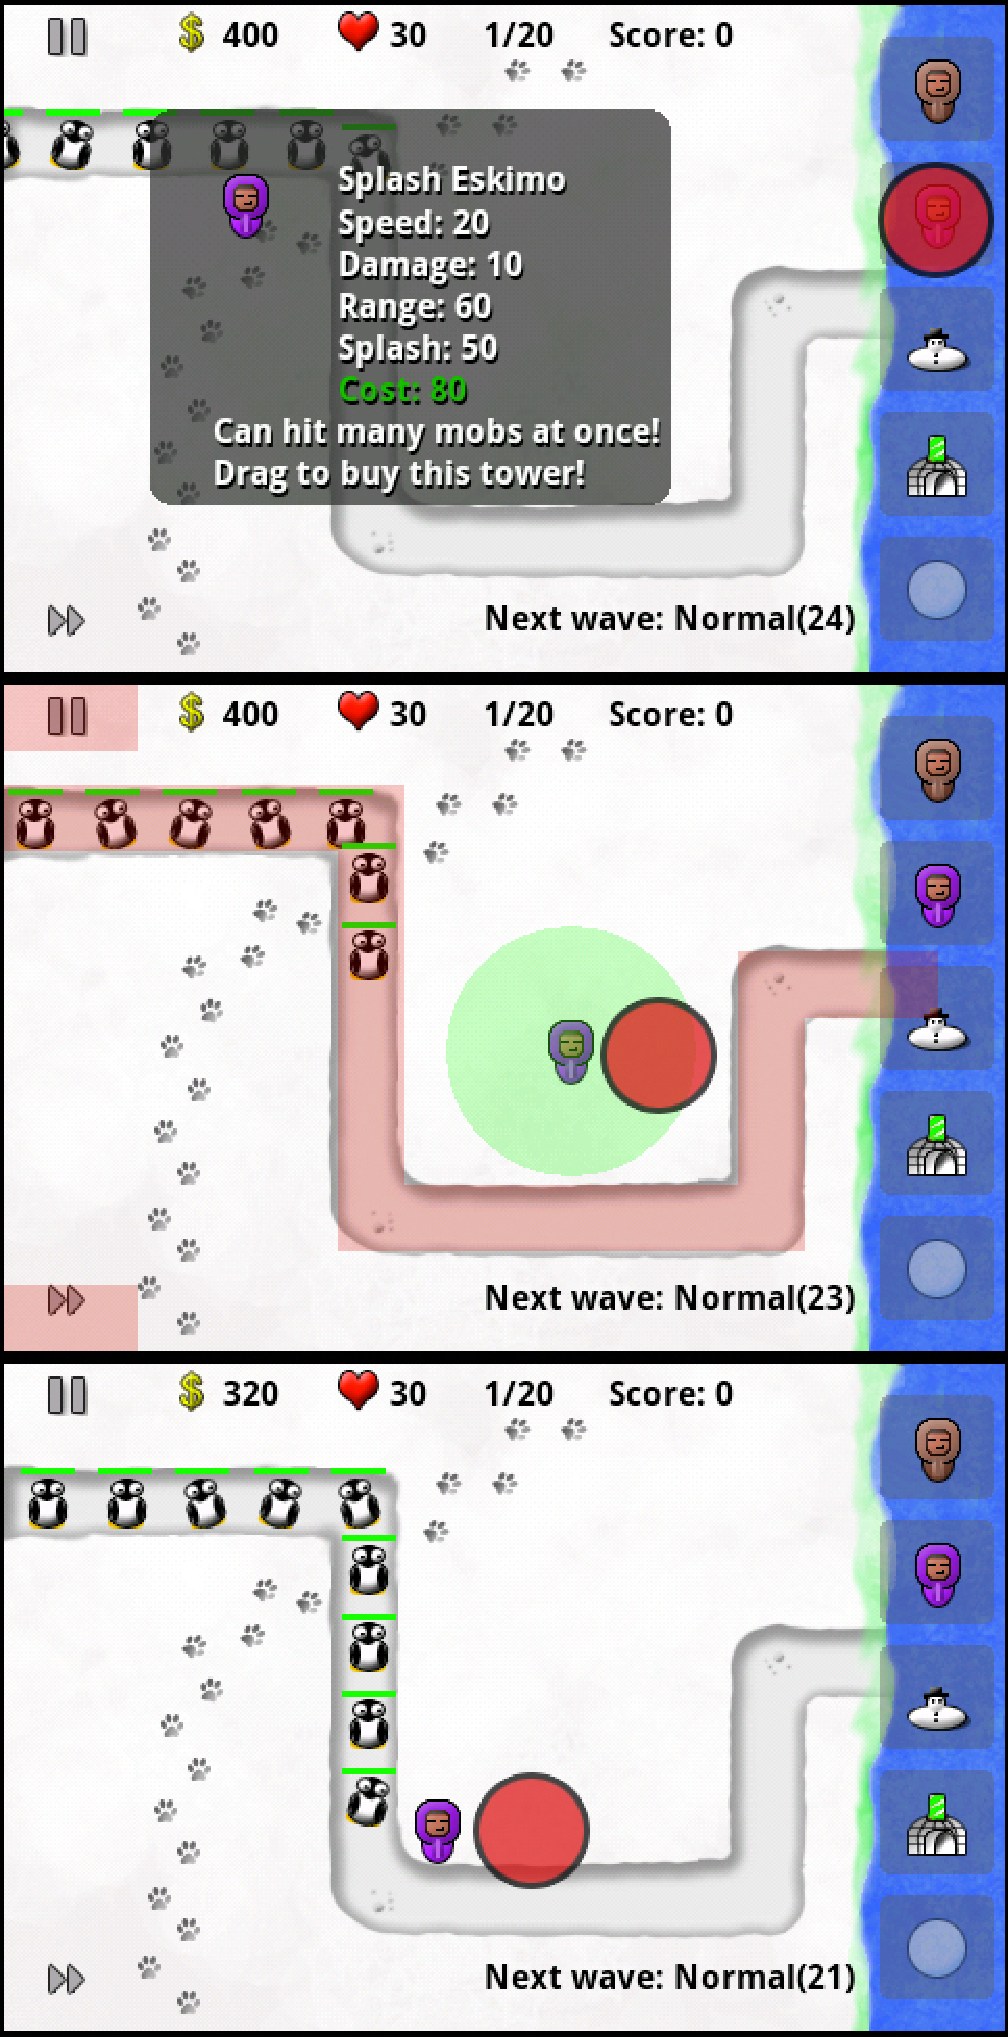
\includegraphics[scale=0.3]{pics/chapters/chapter4/buildertowerallthree}
\end{center}
\caption{Screenshots of a tower being built. The red circle shows where the screen is touched.}
\label{fig:towerPlacement}
\end{figure}
%---------

\clearpage

\subsection{Tower upgrade}

Upgrading a tower requires the user to press the tower on the game field. A tooltip will then be displayed with information about the tower\'s current level and next level attributes. Two buttons are available, one button to sell and another button to upgrade the tower. If the player has enough money to upgrade, the upgrade button is green and if not, the button is red. The colored text indicates how the attributes will change when the tower is upgraded.

When the upgrade tooltip is shown, the game will not be paused. This is not one of the four states that was described earlier. It is a smaller state in STATE\_RUNNING which allows the toolbox to be displayed and the game still be running. The green circle around the tower is also displayed to make the player certain about that he pressed the correct tower.  

If the sell button is pressed, the tooltip will be removed and the tower along with it. The upgrade button will upgrade the tower, changing its attributes and image.

%---------
%- Image upgrade tower
%---------
\begin{figure}[here]
\begin{center}
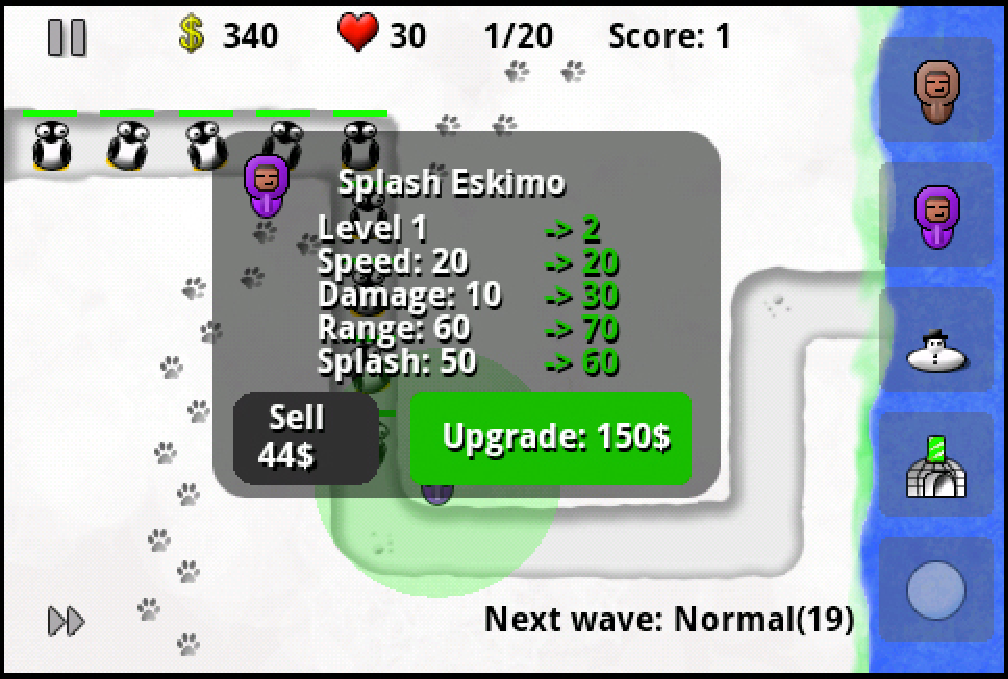
\includegraphics[scale=0.6]{pics/chapters/chapter4/towerupgrade}
\end{center}
\caption{Screenshot of the upgrade window}
\label{fig:towerUpgrade}
\end{figure}
%---------

There are four different types of towers and they all have four different levels of power. The image of the towers reflect this (see figure ~\ref{fig:allTowers}).
\clearpage
%---------
%- Image towers
%---------
\begin{figure}[here]

\begin{center}

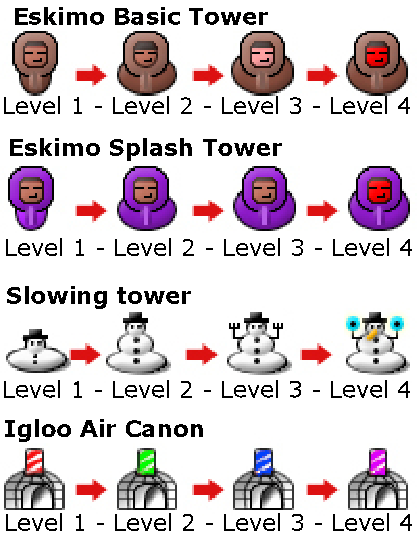
\includegraphics[scale=0.6]{pics/chapters/chapter4/alltowers}

\end{center}

\caption{All towers of the Eskimo Tower Defense}

\label{fig:allTowers}

\end{figure}
%---------

\subsection{Mobs}

There are five different mob types: Penguin, Bear, Polar Bear, Walrus and Flying Penguin (see Figure ~\ref{fig:mobs}). Some of the mobs are animated. This is achieved in the same way as the water splash. A health bar is drawn above the mobs to show the health of each individual mob. This allows the player to get a more detailed idea of how the mobs health is distributed. 

%---------
%- Image mobs
%---------
\begin{figure}[h]
\begin{center}

\includegraphics[scale=0.6]{pics/chapters/chapter4/mobs}
\end{center}
\caption{The different mobs of the game}
\label{fig:mobs}
\end{figure}
%---------

The health bar is not a bitmap but rather two rectangles drawn on the canvas; one for the black background and one for the health. The health-rectangle's length and color is calculated by the health of the mob. The less health a mob has the shorter and redder the bar gets. With full health the health-rectangle is green. The ratio of how much health the mob has is calculated by the following formula:

%--------------
%- Code snippet mob health
%--------------
\begin{figure}[htb]

\begin{small}
\verbatiminput{code/mobHealth.java}
\end{small}

\caption{Caption}
\label{fig:codeExMobHealth}

\end{figure}
%--------------